% Niveau :      PCSI *
% Discipline :  Chimie Orga I
% Mots clés :   Spectrométrie UV-visible, Réactions acidobasiques

\begin{exercise}{Les hydrures du bloc $p$}{2}{MPSI}
{Atomistique,Classification périodique, Structure électronique}{bermu}

\begin{questions}
    
    \questioncours En introduisant dans le détail les concepts utilisés, commenter l'évolution des caractéristiques physiques des hydrures des éléments du bloc $p$ présentés dans la figure et la table ci-dessous.
\end{questions}

    \begin{figure}[H]
        \centering
        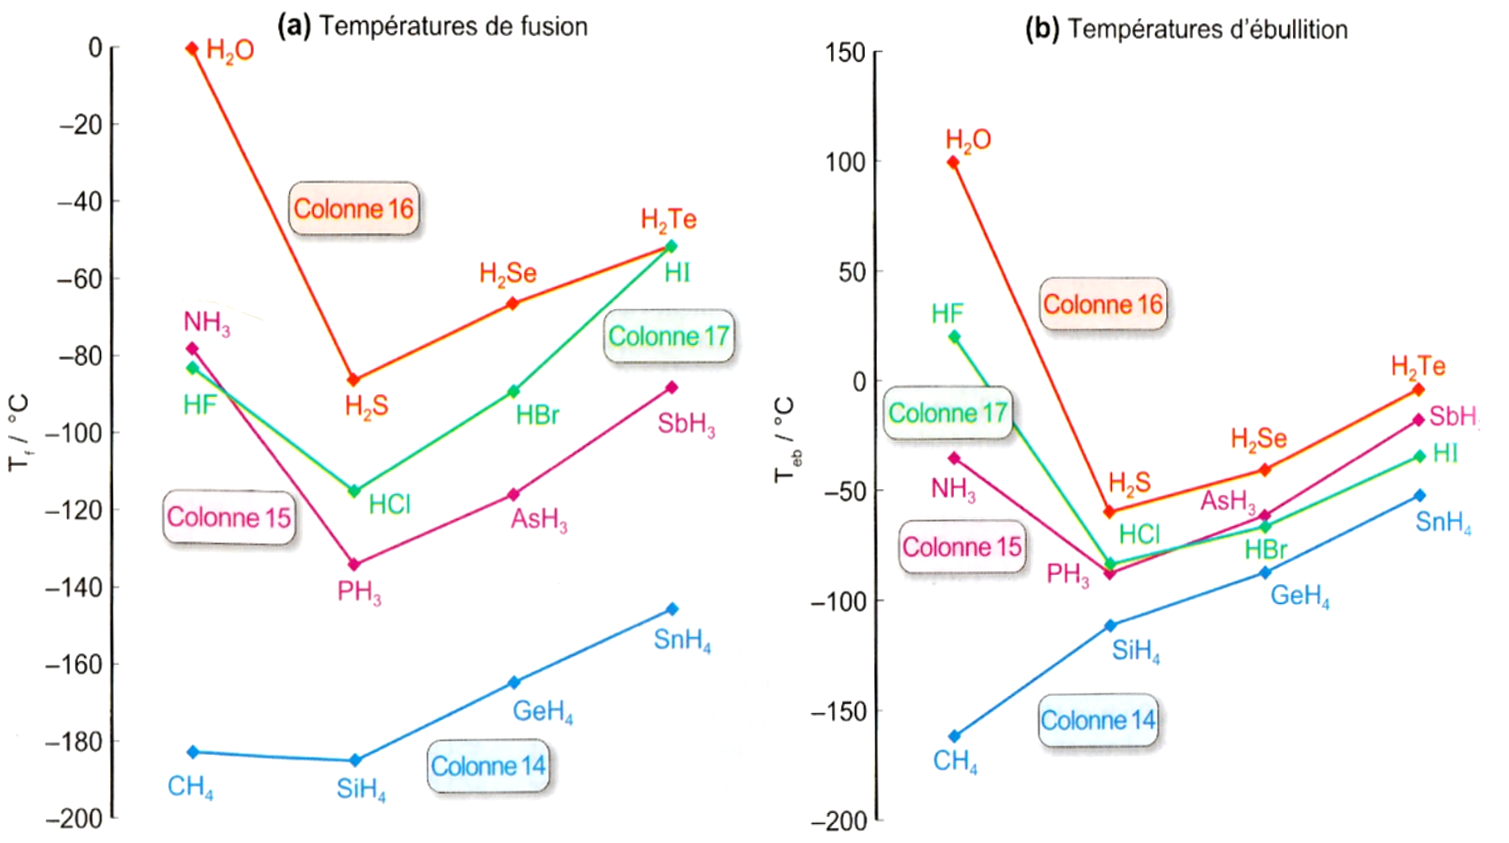
\includegraphics[width=.9\linewidth]{chimie/solvants/hydrures.png}
        \caption{Températures de fusion (a) et d'ébullition (b) des hydrures des éléments du bloc $p$ à pression atmosphérique.}
        \label{fig:hydrures}
    \end{figure}

\end{exercise}

\begin{exercise}{Nitrophénol$\cdot$s}{2}{PCSI}
{Atomistique,Classification périodique, Structure électronique}{bermu}

\begin{questions}
    \questioncours En introduisant dans le détail les concepts utilisés, commenter l'évolution des caractéristiques physiques des différents nitrophénols : ortho, méta et para.
 \end{questions}
 
\begin{table}[H]  
	\setchemfig{chemfig style={scale=0.75}, atom style={scale=0.75}}
    \begin{tabularx}{.8\linewidth}{r|CCC}
        & \chemfig{**6(---(-OH)-(-NO_3)---)}    %[scale=0.75][scale=0.75]
        & \chemfig{**6(--(-OH)--(-NO_3)---)}
        & \chemfig{**6(-(-OH)---(-NO_3)---)}\\
         & ortho & méta & para \\ \hline\hline
        Apparence & cristaux jaunes & cristaux incolores & aiguilles incolores \\
Point de fusion ($^\circ$C) & 44 & 97 & 114 \\
Point d'ébullition ($^\circ$C) & 214 & 194 & > 260 \\
pK$_a$ & 7,21 & 8,38 & 7,16 \\
Solubilité dans l'eau (g$\cdot$L$^{-1}$) & 2,1 & 13,5 & 14,8 \\ \hline
    \end{tabularx}

    \caption{Comparaisons de propriétés physiques des différents nitrophénols. (CTNP).}
\end{table}
\end{exercise}

\begin{exercise}{Catalyse par transfert de phase}{2}{MPSI}
{Atomistique,Classification périodique, Structure électronique}{bermu}

On s'intéresse à la réaction suivante entre les ions hypochlorite et l'alcool benzylique :
$$\mathrm{Ph-CH_2-OH + C\ell O^\ominus \quad\longrightarrow\quad Ph-CH=O + C\ell^\ominus + H_2O}$$

L'ion hypochlorite est dissout dans l'eau alors que l'acool est dissout dans un solvant organique : l'éthanoate d'étyle $\mathrm{CH_3-CO-O-CH_2-CH_3}$.

\begin{questions}
    \questioncours Rappeler le processus de solubilisation et justifier les deux solvants utilisés.
    
    \question En l'état, la réaction peut-elle se faire ? Pourquoi ne pas avoir utilisé un alcool comme milieu réactionnel ?
    
\uplevel{On introduit en petite quantités le sel TBAF de formule ionique $\mathrm{(C_4H_9)_4-N^\oplus + F^\ominus}$ .}
    
    \question Expliquer qu'après ajout de TBAF, la réaction à lieu.
    
\end{questions}

\end{exercise}

% Niveau :      PCSI *
% Discipline :  Chimie Orga I
% Mots clés :   Spectrométrie UV-visible, Réactions acidobasiques

\begin{exercise}{Chimie click, chimie verte}{2}{PCSI}
{Solvants}{bermu}



\begin{questions}
    \questioncours Différentes étapes de la solvatation d'un soluté dans un solvant. \\
    On illustrera la question d'exemple en rentrant dans le détail des différents types de solvants.

\begin{EnvUplevel}

Une des tendances actuelles en chimie de synthèse est la chimie click au micro-onde de la réaction de Biginelli :
\begin{center}
    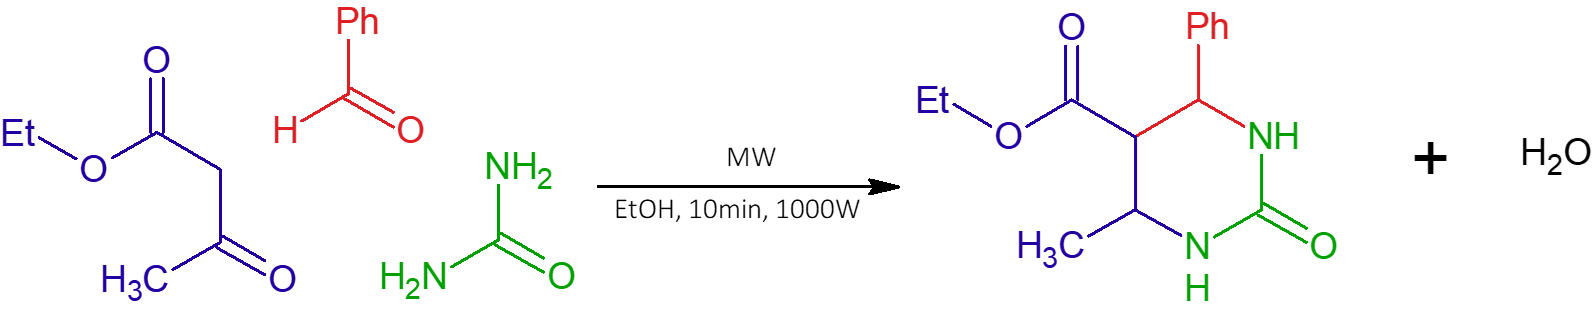
\includegraphics[width=.9\linewidth]{chimie/solvants/click.png}
\end{center}

\end{EnvUplevel}

    \question Justifier le choix de l'éthanol comme solvant de cette réaction.
    
\uplevel{Cette réaction  est activée grâce aux micro-ondes. Pour rappel, les fours à micro-ondes excitent à une fréquence spécifique pour exciter les molécules d'eau.}
    
    \question  Justifier que l'éthanol est excité par les micro-ondes et que cela permet de catalyser la réaction.
    
    \uplevel{Normalement, une telle réaction se ferait en plusieurs d'étapes dans plusieurs solvants.}
    
    \question Conclure quant aux gains écologique pour réaliser cette réaction. Pour information les 12 principes de la chimie verte ci-dessous.
    
    \begin{table}[H]
        \centering
        \begin{tabular}{ll}
            \\\hline\hline
            1. Prévention : moins de déchets ; &
            7. Matières renouvelables  ;\\
            2. Économie d'atomes : moins de sous-produits ; &
            8. Schéma de synthèse efficace ;\\
            3. Réactif doux : pas de substances toxiques ; &
            9. Catalyse ;\\
            4. Réduire la toxicité des produits utilisés ; &
            10. Produits biodégradables ;\\
            5. Pas de substances auxiliaires (solvants...) &
            11. Contrôle des conditions de réaction ; \\
            6. Conditions douces : CNTP ; &
            12. Réduire les risques d'accidents. \\ \hline
        \end{tabular}
        \caption{Principes de la chimie verte}
    \end{table}
\end{questions}
\end{exercise}